\documentclass[tikz,border=4pt]{standalone}
\usepackage[T1]{fontenc}
\usepackage[utf8]{inputenc}
\usepackage{lmodern}
\usepackage{amsmath,amssymb,mathtools,bm}
\usepackage{graphicx}
\usepackage{booktabs}
\usepackage{array}

\usepackage{tikz}
\usetikzlibrary{arrows.meta,positioning,calc,decorations.pathreplacing,backgrounds,fit,
                shapes.geometric,shapes.misc}
\usepackage{pgfplots}
\pgfplotsset{compat=1.18}
\usepgfplotslibrary{groupplots}

% ---------------------------------------------------------------------
%  PALETTE (light theme of the mid-term presentation)
% ---------------------------------------------------------------------
\definecolor{ink}{RGB}{30,41,59}
\definecolor{muted}{RGB}{100,116,139}
\definecolor{rule}{RGB}{203,213,225}
\definecolor{primary}{RGB}{21,101,146}
\definecolor{teal}{RGB}{34,148,136}
\definecolor{amber}{RGB}{224,122,63}
\definecolor{plum}{RGB}{124,92,168}
\definecolor{panel}{RGB}{238,243,247}
\definecolor{panel2}{RGB}{233,242,240}
\definecolor{cardln}{RGB}{210,222,232}
% methods (the same colours as in every result figure of the report)
\definecolor{cref}{HTML}{2CA02C}
\definecolor{cnone}{HTML}{D62728}
\definecolor{cwhole}{HTML}{FF7F0E}
\definecolor{csub}{HTML}{8C564B}
\definecolor{cocc}{HTML}{1F77B4}
\definecolor{cjoint}{HTML}{9467BD}
% terrain / DEM, unknown scene and data
\definecolor{terrain}{RGB}{120,90,60}
\definecolor{terrainfill}{RGB}{235,228,214}
\definecolor{cunk}{HTML}{C62828}
\definecolor{cdat}{HTML}{1565C0}
% the four channels (one hue, light to dark)
\definecolor{chA}{HTML}{0D47A1}
\definecolor{chB}{HTML}{1E6FCC}
\definecolor{chC}{HTML}{4A94DE}
\definecolor{chD}{HTML}{90C2F0}

\renewcommand{\familydefault}{\sfdefault}
\usepackage{xcolor}
% notation
\newcommand{\dC}{\Delta C_0}
\newcommand{\Nrx}{N_{\mathrm{rx}}}
\newcommand{\PRF}{\mathrm{PRF}}
\newcommand{\PRFop}{\mathrm{PRF}_{\mathrm{op}}}
\newcommand{\bxt}{b_{\mathrm{xt}}}
\newcommand{\bat}{b_{\mathrm{at}}}
\newcommand{\bxti}{b_{\mathrm{xt},i}}
\newcommand{\bati}{b_{\mathrm{at},i}}
\newcommand{\Ba}{B_{\mathrm{a}}}
\newcommand{\jj}{\mathrm{j}}
\newcommand{\ee}{\mathrm{e}}
\newcommand{\Hm}{^{\mathsf H}}
\newcommand{\T}{^{\mathsf T}}
\newcommand{\F}{\mathbf F}
\newcommand{\D}{\mathcal D}
\newcommand{\vg}{\bm g}
\newcommand{\vgh}{\hat{\bm g}}
\newcommand{\gs}{g}
\newcommand{\sv}{{\color{cdat}\bm s}}
\newcommand{\ssv}{{\color{cdat}s}}

\tikzset{
  >={Stealth[length=2.4mm]},
  box/.style   ={rounded corners=3pt,draw=primary,line width=0.9pt,fill=panel,
                 text=ink,align=center,inner sep=4pt,font=\scriptsize},
  tbox/.style  ={rounded corners=3pt,draw=teal,line width=0.9pt,fill=panel2,
                 text=ink,align=center,inner sep=4pt,font=\scriptsize},
  abox/.style  ={rounded corners=3pt,draw=amber,line width=0.9pt,fill=amber!12,
                 text=ink,align=center,inner sep=4pt,font=\scriptsize},
  pbox/.style  ={rounded corners=3pt,draw=plum,line width=0.9pt,fill=plum!10,
                 text=ink,align=center,inner sep=4pt,font=\scriptsize},
  gbox/.style  ={rounded corners=3pt,draw=muted,line width=0.7pt,fill=white,
                 text=ink,align=center,inner sep=4pt,font=\scriptsize},
  dbox/.style  ={rounded corners=3pt,draw=terrain,line width=0.8pt,fill=terrainfill,
                 text=ink,align=center,inner sep=4pt,font=\scriptsize},
  dec/.style   ={diamond,aspect=2.3,draw=amber,line width=0.8pt,fill=amber!14,
                 text=ink,align=center,inner sep=1pt,font=\tiny},
  stepn/.style ={circle,fill=amber,text=white,font=\tiny\bfseries\sffamily,inner sep=0.6pt,minimum size=3.9mm},
  arr/.style   ={-{Stealth[length=2.2mm]},line width=0.9pt,draw=muted},
  bx/.style    ={rounded corners=2pt,line width=0.8pt,align=center,inner sep=2.5pt,text width=#1},
  bx/.default=3.2cm,
  lane/.style  ={rounded corners=5pt,line width=0.7pt},
  ln/.style    ={anchor=north,align=center,font=\footnotesize},
  tarr/.style  ={-{Stealth[length=2.2mm]},line width=1.0pt,draw=teal},
  aarr/.style  ={-{Stealth[length=2.2mm]},line width=1.0pt,draw=amber},
  parr/.style  ={-{Stealth[length=2.2mm]},line width=1.0pt,draw=plum},
  cota/.style  ={<->,line width=0.5pt,draw=muted},
  brc/.style   ={decorate,decoration={brace,amplitude=4pt},draw=muted,line width=0.6pt},
  nota/.style  ={font=\scriptsize,text=muted,align=center},
  % operators of the joint model, coloured by the domain in which they act
  op/.style    ={draw=muted,fill=white,rounded corners=2pt,align=center,inner sep=2.5pt,
                 minimum height=8mm,minimum width=10mm,font=\small,line width=0.6pt},
  opx/.style   ={op,draw=teal,fill=panel2},      % position (focused line)
  opf/.style   ={op,draw=primary,fill=panel},    % Doppler frequency
  opt/.style   ={op,draw=amber,fill=amber!10},   % time (raw channel line)
  sat/.style   ={circle,draw=ink,fill=white,line width=0.8pt,inner sep=2pt},
}


% ---------------------------------------------------------------------------------------------- helpers
\tikzset{
  invisible/.style={opacity=0,text opacity=0},
  visible on/.style={alt={#1{}{invisible}}},
  alt/.code args={<#1>#2#3}{\alt<#1>{\pgfkeysalso{#2}}{\pgfkeysalso{#3}}},
  gvisible on/.style={alt={#1{}{transparency group,opacity=0}}},
  nohyph/.style={execute at begin node={\hyphenpenalty=10000\exhyphenpenalty=10000}},
  pillst/.style={rounded corners=4.5pt,inner xsep=4.5pt,inner ysep=1.6pt,font=\scriptsize\sffamily\bfseries},
  lbl/.style={font=\scriptsize,text=ink},
  mlbl/.style={font=\scriptsize,text=muted},
}
\definecolor{sl0}{HTML}{E2E8F0}\definecolor{sl1}{HTML}{CBD5E1}\definecolor{sl2}{HTML}{94A3B8}\definecolor{sl3}{HTML}{64748B}
\newcommand{\pilltw}{\tikz[baseline=-0.62ex]\node[pillst,fill=primary!14,text=primary]{this work};}
\newcommand{\cfg}[1]{\framesubtitle{#1}}
\newcommand{\cfgp}[2]{\framesubtitle{#2\hfill#1}}
\newcommand{\dt}{\enspace$\cdot$\enspace}
\newcommand{\lyr}[2]{\node<#1>[anchor=north west,inner sep=0pt] at (0,0) {\includegraphics{figures/v20/#2}};}
% phase dial: centre (#1,#2), radius #3; arrow at #4 degrees clockwise from 12 o'clock, colour #5
\newcommand{\dialbase}[3]{\draw[rule,line width=0.6pt,fill=white] (#1,#2) circle (#3);
  \draw[muted,line width=0.6pt] (#1,#2+#3) -- (#1,#2+0.78*#3);}
\newcommand{\dialarc}[5]{\draw[#5,line width=0.8pt] ($(#1,#2)+(90:{0.58*#3})$) arc[start angle=90,end angle={90-(#4)},radius={0.58*#3}];}
\newcommand{\dialarrow}[5]{\draw[-{Stealth[length=1.9mm,width=1.8mm]},line width=1.2pt,#5] (#1,#2) -- ++({90-(#4)}:{0.84*#3});}
% slide 9: the scatterer on the iso-range arc of the Tx (angle #1 seen from the Tx), #2 > 0: label it
\newcommand{\scat}[2]{%
  \coordinate (P) at ($(Tx)+(#1:\rr)$);
  \draw[primary,line width=0.9pt] (Tx) -- (P);
  \draw[chB,line width=0.9pt] (Rx) -- (P);
  \ifnum#2>1 \draw[cota] (P |- 0,\zg) -- node[right=-1pt]{$h$} (P); \fi
  \ifnum#2>0 \node[anchor=west] at ($(P)+(0.25,0.1)$) {scatterer}; \fi
  \fill[ink] (P) circle (2.3pt);}


% ---------------------------------------------------------------------------------------------- v28 helpers
% styles of the joint algorithm (overview, stage slides and closing)
\tikzset{
  pa/.style={rounded corners=2pt,line width=0.8pt,draw=ink!55,fill=white,align=center,text width=2.35cm,
             inner sep=2.2pt,minimum height=1.55cm,nohyph},
  lo/.style={rounded corners=2pt,line width=0.8pt,draw=primary,fill=panel,align=center,text width=2.1cm,
             inner sep=2.2pt,minimum height=1.0cm,nohyph},
  fi/.style={rounded corners=2pt,line width=0.8pt,draw=plum,fill=plum!10,align=center,text width=3.0cm,inner sep=2.2pt,
             nohyph},
  io/.style={rounded corners=2pt,line width=0.8pt,draw=muted,fill=muted!8,align=center,inner sep=2.2pt,nohyph},
  bd/.style={circle,fill=amber,text=white,font=\scriptsize\bfseries\sffamily,inner sep=0pt,minimum size=5.0mm},
  parr2/.style={-{Stealth[length=2.2mm]},line width=1.0pt,draw=primary},
  lanelab/.style={anchor=west,align=left,text width=2.0cm,font=\footnotesize\bfseries,nohyph},
}
\newcommand{\jointstyles}{}
% "you are here": a thumbnail of the overview (three lanes) in the top-right corner, below the title rule;
% #1 = comma list of the lit cells: P1,P2,P3,P4,L (the loop),F1,F2
\makeatletter
\newcommand{\yhcell}[5]{% name, x, y, width, label
  \edef\yh@do{\noexpand\in@{,#1,}{,\yhlist,}}\yh@do
  \ifin@\node[draw=amber,fill=amber,text=white,minimum width=#4cm,minimum height=0.27cm,inner sep=0pt,rounded corners=1pt]
     at (#2,#3) {#5};
  \else\node[draw=rule,fill=white,text=muted,minimum width=#4cm,minimum height=0.27cm,inner sep=0pt,rounded corners=1pt]
     at (#2,#3) {#5};\fi}
\makeatother
\newcommand{\youarehere}[1]{%
  \def\yhlist{#1}%
  \begin{tikzpicture}[remember picture,overlay]
    \begin{scope}[shift={([xshift=-3.25cm,yshift=-2.75cm]current page.north east)},x=1cm,y=1cm,
                  font=\fontsize{5}{5}\selectfont\sffamily\bfseries]
      \fill[muted!5,rounded corners=1.5pt] (0,0.9) rectangle (2.65,1.3); \draw[ink!40,rounded corners=1.5pt,line width=0.4pt] (0,0.9) rectangle (2.65,1.3);
      \fill[panel!60,rounded corners=1.5pt] (0,0.45) rectangle (2.65,0.85); \draw[primary,rounded corners=1.5pt,line width=0.4pt] (0,0.45) rectangle (2.65,0.85);
      \fill[plum!6,rounded corners=1.5pt] (0,0) rectangle (2.65,0.4); \draw[plum,rounded corners=1.5pt,line width=0.4pt] (0,0) rectangle (2.65,0.4);
      \yhcell{P1}{0.42}{1.1}{0.52}{P1}\yhcell{P2}{1.02}{1.1}{0.52}{P2}\yhcell{P3}{1.62}{1.1}{0.52}{P3}\yhcell{P4}{2.22}{1.1}{0.52}{P4}
      \yhcell{L}{1.32}{0.65}{2.32}{S1--S3 loop}
      \yhcell{F1}{0.72}{0.2}{1.12}{F1}\yhcell{F2}{1.92}{0.2}{1.12}{F2}
    \end{scope}
  \end{tikzpicture}}

% ---- v28: the five factors of the model s_i = D H_i K Psi_i g, one colour each, the same on every joint slide
%      (never red / green / purple: those mean standard / reference / joint reconstruction)
\colorlet{fD}{amber!88!black}\colorlet{fH}{primary}\definecolor{fK}{HTML}{5B6B85}\colorlet{fP}{terrain}\colorlet{fG}{ink}
\newcommand{\fD}{{\color{fD}D}}\newcommand{\fH}{{\color{fH}H_i}}\newcommand{\fK}{{\color{fK}K}}
\newcommand{\fKi}{{\color{fK}K_i}}\newcommand{\fP}{{\color{fP}\Psi_i}}
\newcommand{\modelA}{\mathbf A_i=\fD\cdot\fKi\cdot\fP}
% ---- v28: the simulation parameters, the same grey block under the title of every result slide; #1 = what is
%      specific to the slide
\newcommand{\simline}{$N_{\mathrm{rx}}=4$ (Rx0 $=$ Tx)\dt 500\,Hz each (2000\,Hz together)\dt
  $\bxt=300,\ 119.8,\ 100.5$\,m\dt $\lambda=0.25$\,m\dt $v=7689$\,m/s\dt $r_0=766$\,km}
\newcommand{\simcfg}[1]{\framesubtitle{\simline\\ look angle $20^\circ$\dt $\Ba=1235$\,Hz\dt #1}}

% standalone: every build step shown
\tikzset{visible on/.style={},gvisible on/.style={}}
\providecommand{\vstrip}[5]{\foreach \c in {1,...,#3}
  \draw[#5,line width=0.5pt] ({#1+(\c-1)*#4},{#2-0.17}) rectangle ({#1+\c*#4},{#2+0.17});}

% Where H_i and K come from: the range curves of the h = 0 point give H_i; the echo of the same point, one radar alone, gives K = its FFT; K H_i is that point at receiver i
\begin{document}
\begin{tikzpicture}[x=1cm,y=1cm,font=\footnotesize,
      kc/.style={anchor=north,align=center,font=\footnotesize,inner sep=1pt,nohyph},
      ar/.style={-{Stealth[length=2.0mm]},line width=0.9pt,draw=ink!70}]
    \jointstyles
    \path (-0.1,-0.75) rectangle (15.0,5.5);
    % ================= step 1: P1, the range curves of the h = 0 point -> the three terms of H_i
    
    \node[anchor=west,font=\footnotesize,align=left] at (0.45,5.3)
      {the ranges of the $h=0$ point give each channel its filter $\fH$\enspace{\color{muted}($|{\color{fH}H_i}|=1$: only a phase)}};
    \def\ox{0.45}\def\oy{3.45}
    \draw[->,ink] (\ox,\oy) -- (\ox+4.2,\oy) node[right]{$t_a$};
    \draw[->,ink] (\ox,\oy) -- (\ox,\oy+1.55);
    \node[rotate=90,anchor=south,font=\footnotesize] at (\ox-0.05,\oy+0.78) {range};
    \draw[muted!80,line width=1.0pt] plot[domain=-1.55:1.6,samples=40,smooth] ({\ox+1.9+\x},{\oy+0.3+0.22*\x*\x});
    \draw[chB,line width=1.1pt] plot[domain=-1.3:1.85,samples=40,smooth] ({\ox+1.9+\x},{\oy+0.95+0.2*(\x-0.7)^2});
    \node[anchor=west,text=muted,font=\footnotesize,align=left] at (\ox+3.55,\oy+0.62) {one radar\\ alone: $2r_{T_x}$};
    \node[anchor=west,text=chB,font=\footnotesize,align=left] at (\ox+3.75,\oy+1.4) {channel $i$:\\ $r_{T_x}+r_{R_x,i}$};
    \draw[muted,densely dotted] (\ox+1.9,\oy+0.3) -- (\ox+3.0,\oy+0.3);
    \draw[cota,draw=amber,line width=0.8pt] (\ox+2.8,\oy+0.3) -- (\ox+2.8,\oy+0.95);
    \node[anchor=west,text=amber!85!black,font=\footnotesize\bfseries,inner sep=1pt] at (\ox+2.9,\oy+0.55) {$C_0$};
    \draw[muted,densely dotted] (\ox+2.6,\oy+0.95) -- (\ox+2.6,\oy-0.3);
    \draw[muted,densely dotted] (\ox+1.9,\oy+0.3) -- (\ox+1.9,\oy-0.3);
    \draw[cota,draw=primary,line width=0.8pt] (\ox+1.9,\oy-0.25) -- (\ox+2.6,\oy-0.25);
    \node[anchor=west,text=primary,font=\footnotesize\bfseries] at (\ox+2.65,\oy-0.25) {$\Delta t-C_1$};
    \node[anchor=east,text=muted,font=\footnotesize] at (\ox+1.85,\oy-0.25) {$t_a=0$};
    \node[anchor=west,text=plum,font=\footnotesize\bfseries] at (\ox+0.3,\oy+1.12) {$C_2$};
    \node[box,font=\small,anchor=north,inner sep=4pt] (hbox) at (10.95,4.32) {${\color{fH}H_i(f)}=\exp\Big(-\jj2\pi\Big[
      \textcolor{amber!85!black}{\underbrace{\textcolor{ink}{\tfrac{C_{0,i}}{\lambda}}}_{\mbox{\footnotesize offset}}}
      +\textcolor{primary}{\underbrace{\textcolor{ink}{(\Delta t_i-C_{1,i})\,f}}_{\mbox{\footnotesize shift}}}
      +\textcolor{plum}{\underbrace{\textcolor{ink}{C_{2,i}\,\lambda f^2}}_{\mbox{\footnotesize bend}}}\Big]\Big)$};
    % ================= step 2: P2, one point at h = 0 seen by one radar alone -> its echo k_0
    \begin{scope}[visible on=<2->]
      \draw[rule,line width=0.5pt] (-0.05,2.95) -- (15.0,2.95);
      
      \node[anchor=west,font=\footnotesize] at (0.45,2.67) {the echo of the $h=0$ point};
      \draw[-{Stealth[length=1.6mm]},ink!60,line width=0.6pt] (0.3,2.15) -- (2.75,2.15) node[right,inner sep=1pt]{$v$};
      \fill[fK!14] (0.6,1.95) -- (1.55,0.55) -- (2.5,1.95) -- cycle;
      \draw[fK!60,line width=0.5pt] (0.6,1.95) -- (1.55,0.55) -- (2.5,1.95);
      \fill[ink] (0.47,1.9) rectangle (0.73,2.06);                    % the radar at the start of the aperture
      \fill[ink!25] (2.37,1.9) rectangle (2.63,2.06);                 % the same radar at its end (faded)
      \draw[ink!70,line width=0.7pt] (0.25,0.55) -- (2.85,0.55);
      \fill[ink!8] (0.25,0.55) rectangle (2.85,0.42);
      \fill[fK] (1.55,0.55) circle (2.4pt);
      \node[font=\footnotesize,fill=fK!14,inner sep=1pt] at (1.55,1.6) {$L_{\mathrm{sa}}$};
      \node[kc,text width=3.0cm] at (1.55,0.35) {one radar (Tx $=$ Rx$_0$),\\ start {\color{muted}and end} of its aperture};
      \draw[ar] (2.9,1.25) -- (3.25,1.25);
      \node[anchor=north west,inner sep=0pt] at (3.3,2.42) {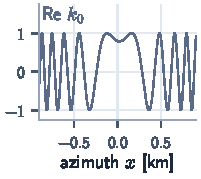
\includegraphics{figures/v29/k_zoom2}};
      \node[kc] at (5.0,-0.55) {its echo $k_0(x)$: a chirp};
    \end{scope}
    % ================= step 3: FFT -> K(f): the band and a quadratic phase
    \begin{scope}[visible on=<3->]
      \draw[ar] (6.75,1.25) -- node[above,font=\footnotesize,inner sep=2pt]{FFT} (7.2,1.25);
      \node[anchor=north west,inner sep=0pt] at (7.25,2.47) {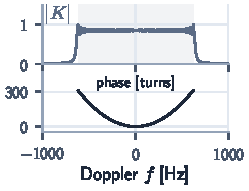
\includegraphics{figures/v29/k_spec3}};
      \node[kc] at (9.35,-0.55) {${\color{fK}K(f)}$: the band $B_{\mathrm a}$, a quadratic phase};
    \end{scope}
    % ================= step 4: x H_i -> the h = 0 point as receiver i records it
    \begin{scope}[visible on=<4->]
      \draw[ar] (11.5,1.25) -- node[above,font=\footnotesize,inner sep=2pt]{$\times{\color{fH}H_i}$} (12.0,1.25);
      \node[rounded corners=3pt,draw=fH,line width=0.9pt,fill=white,align=center,inner xsep=3pt,inner ysep=3pt,
            font=\footnotesize] (ki) at (13.55,1.6)
        {${\color{fK}K_i}={\color{fK}K}\,{\color{fH}H_i}$:\\ the $h=0$ point\\ as receiver $i$ records it};
      \node[anchor=north,align=center,font=\footnotesize,text=muted,inner sep=1pt] at (13.55,0.75) {error vs.\ the directly\\ simulated echo at\\ receiver $i$: $-30$ to $-35$\,dB};
      \node[anchor=east,font=\footnotesize\bfseries,text=ink] at (15.0,2.67)
        {$K$: one flat point, simulated once.\enspace ${\color{fH}H_i}$: moves it to receiver $i$.};
    \end{scope}
  \end{tikzpicture}
\end{document}
